%%%% PROCESAR con PdfLaTeX !!!!!


\documentclass[12pt]{book}
\usepackage{geometry}\geometry{top=2cm,bottom=2cm,left=3cm,right=3cm}
\usepackage{amssymb}
\usepackage{amsmath}
\usepackage{graphicx}
\usepackage{txfonts}




\begin{document}
\thispagestyle{empty}

\begin {center}

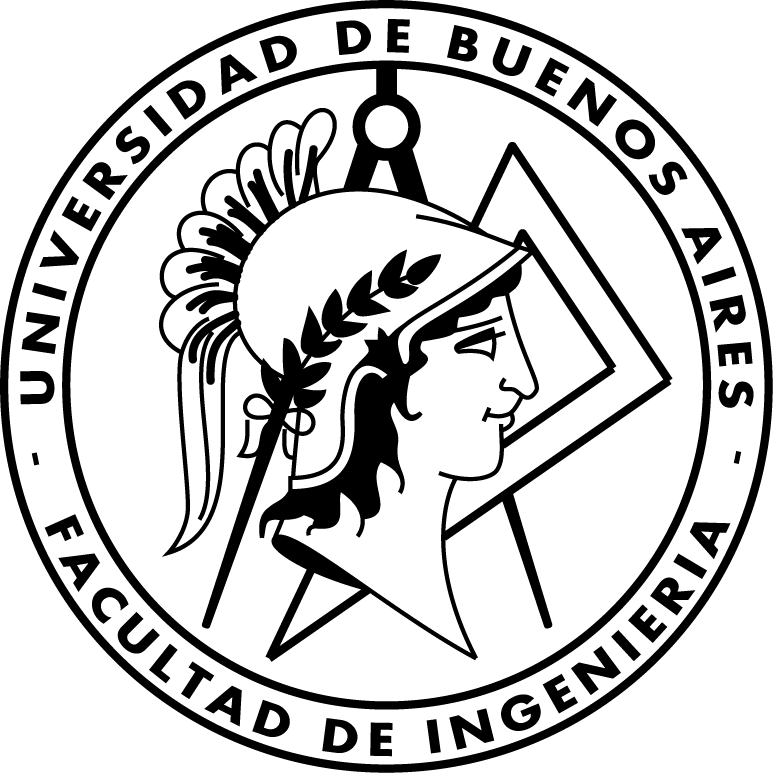
\includegraphics[scale=.4]{Logo-fiuba_big.png}

\medskip
UNIVERSIDAD DE BUENOS AIRES

Facultad de Ingenier\'ia

Departamento de Agrimensura y Geodesia


\vspace{3cm}


\textbf{\large 70.03. Medios de Representación A}

\vspace{2cm}


Este es un modesto aporte para los alumnos de la f\'acultad de ingenier\'ia  de la UBA de la carrera de  ingenier\'ia civil.\\
De ninguna man\'era pretende ser una gu\'ia de estudio, ni remplaza las clases presenciales, el material oficial de la catedra esta disponible en el web site de la m\'ateria.
\\

\end {center}


\vspace{2.5cm}

\noindent Autor:\,	Isaac Edgar Camacho Ocampo
 
\noindent Carrera:\,	Ingeniería Civil

\vspace{1cm}

\vspace{1cm}

\noindent Buenos Aires, 2019

\newpage


\tableofcontents

\chapter{Clase 1}
\section{Material a utilizar + Bibliografía.}
\section{TP0 – Explicación.}
\section{Formatos de Hojas, Recuadro, Rótulo, Grosor de Líneas.}
\subsection{Letras Norma IRAM.}
\subsection{Doblado de Láminas.}
\subsection{Escala.}
\subsection{Trazado Previo y Definitivo.}
\subsection{Cotas.}
\subsection{Trazados Geométricos – Empalmes – Tangentes. Lámina 1C: Empalmes.}
\subsection{Cicloides: Concepto. Cicloide Normal, Corta y Larga. Epicicloides. Lámina 1B: Cicloides.}
\subsection{Curvas Cónicas: Elipses, Parábolas, Hipérbolas. Lámina 1A: Cónicas.}
\subsection{Bibliografía: Di Lorenzo: Tomo 2, Cap. 1.}

\chapter{Clase 2 }

\section{Otros conceptos sobre geometría, curvas y trazados geométricos.}
\section{Sistemas de Proyección - Clasificación}
\subsection{Sistema Monge: Generalidades. Cuadrantes. Cota y Alejamiento. Proyecciones del Punto.}
\subsection{Proyecciones de las Rectas. Posiciones particulares de puntos y rectas.}
\subsection{Trazas de las rectas.}
\subsection{Condición de pertenencia de punto a recta.}
\subsection{Sistema Monge: Planos: Pertenencia de Recta a Plano.}
\subsection{Sistema Monge: Trazas del Plano. Posiciones particulares del Plano.}
\subsection{Lámina 2B: Método Monge - Trazas.}
\subsection{AutoCAD: Introducción. Comandos básicos de dibujo y modificación.}
\subsection{Lámina 2A: Método Monge - Triedro.}
\subsection{Bibliografía: Di Lorenzo: Tomo 2, Cap. 1.}

\chapter{Clase 3}
\section{Repaso de Proyecciones de Recta y Plano. Posiciones Particulares. Pertenencia y Trazas.}
\section{Problemas de Posición.}
\section{Representación de Planos (todas las formas).}
\section{Tercera Proyección de los elementos geométricos.}
\section{Lámina 2C: Problemas de Posición – Planos.}
\section{Rectas Alabeadas – Visibilidad.}
\section{Lámina 2D Problemas de Posición – Caños.}
\section{Bibliografía: Di Lorenzo: Tomo 1, Cap. 2 y Tomo 1, Apéndice.}

\chapter{Clase 4}
\section{Intersecciones: Recta c/ Plano y Plano c/ Plano.}
\section{Planos auxiliares Proyectantes.}
\section{Recta Normal.}
\section{Lámina 3A: Intersecciones.}
\section{Lámina 3B: Intersecciones.}
\section{Bibliografía: Di Lorenzo: Tomo 1, Cap. 3 y 4.}

\chapter{Clase 5 }

\section{Magnitud: Verdadera Magnitud.}
\section{Distancias y ángulos.}
\section{Giros, Abatimientos y Cambios de Plano de Proyección.}
\section{Lámina 4A: Problemas de Magnitud.}
\section{Lámina 4BC: Problemas de Magnitud – Cubierta Laminar.}
\section{Bibliografía: Di Lorenzo: Tomo 1, Cap. 3 y 4.}


\chapter{Clase 6 }
\section{Repaso de Magnitud: Distancias y ángulos. Giros, Abatimientos y CPP.}
\section{Lámina 4D: Problemas de Magnitud.}
\section{TP2 – Entrega Preliminar}
\section{TP4 - Explicación}
\section{Homología.}
\section{Figuras Planas.}
\section{Bibliografía: Di Lorenzo: Tomo 1, Cap. 3, 4, 7 y 13.}

\chapter{Clase 6 }
\section{Homología.}
\section{Figuras Planas.}
\section{Representación de Cuerpos.}
\section{Lámina 5: Figuras Planas y Cuerpos (Tuerca).}
\section{Bibliografía: Di Lorenzo: Tomo 1, Cap. 7 y 13.}

\chapter{Clase 8}
\section{Representación de Cuerpos (continuación).}
\section{Sección Plana.}
\section{Desarrollo de Cuerpos Rectos.}
\section{Lámina 6: Figuras Planas y Cuerpos (Tolva).}
\section{TP1 – Entrega Definitiva}
\section{Bibliografía: Di Lorenzo: Tomo 1, Cap. 7y Tomo 2, Cap. 7.}

\chapter{Clase 9}
\section{Sistema de Proyecciones Acotadas.}
\section{Lámina 7: Superficies Topográficas.}
\section{Ejemplos de Aplicación Práctica.}
\section{Ejercicios de Representación de cuerpos en Proyecciones Acotadas.}
\section{TP3 – Explicación.}
\section{TP2 – Entrega Definitiva}
\section{Representación y Desarrollo de Cuerpos Oblicuos.}
\section{Esfera. Secciones con elementos geométricos.}
\section{Bibliografía: Di Lorenzo: Tomo 1, Cap. 7 y 11, Tomo 2, Cap. 7.}

\chapter{Clase 10}
\section{Intersección de Superficies.}
\section{Lámina 9: Intersección de Cuerpos.}
\section{Ejercicios de Cuerpos, Sección plana y Desarrollo.}
\section{TP3 – Entrega Preliminar.}
\section{Bibliografía: Di Lorenzo: Tomo 1, Cap. 11. Y Tomo 2, Cap. 7}

\chapter{Clase 11}
\section{Curvas Alabeadas.}
\section{Hélice Cilíndrica y Helicoide. Lámina 8AB: Hélice y Helicoide.}
\section{Lámina 8CD: Tobogán y Tobogán Desarrollo.}
\section{TP4 – Entrega Preliminar.}
\section{Bibliografía: Di Lorenzo: Tomo 2, Cap. 6 y 11.}

\chapter{Clase 12}
\section{Perspectivas.}
\section{Documentación de Proyecto y Obra.}
\section{Repaso general.}
\section{TP3 – Entrega Definitiva.}
\section{TP4 – Entrega Definitiva.}
\section{Bibliografía: Di Lorenzo: Tomo 2, Cap. 6 y 11.}


\end{document}
